\section{Design analysis and concept diagrams}
Description of issues related to the design of the product:
- Description of concepts, requirements and features of the product
- Review of motivations for making the design decisions
- Indicate the primary features of the design that are the most creative and original

\subsection{Materials}
For this project we got a bunch of different plast materials from RIAS, in order to find some material that might be cheaper, and better that acrylic, since acrylic have tendency to be brittle, this becomes worse when it has been laser cut.
all of the plastic was thermoplastic, which is a term that is used in the laser industri to indicate that it can be laser c ut.
for the laser cutter we 
PEHD
\begin{figure}[h]
	\begin{center}
		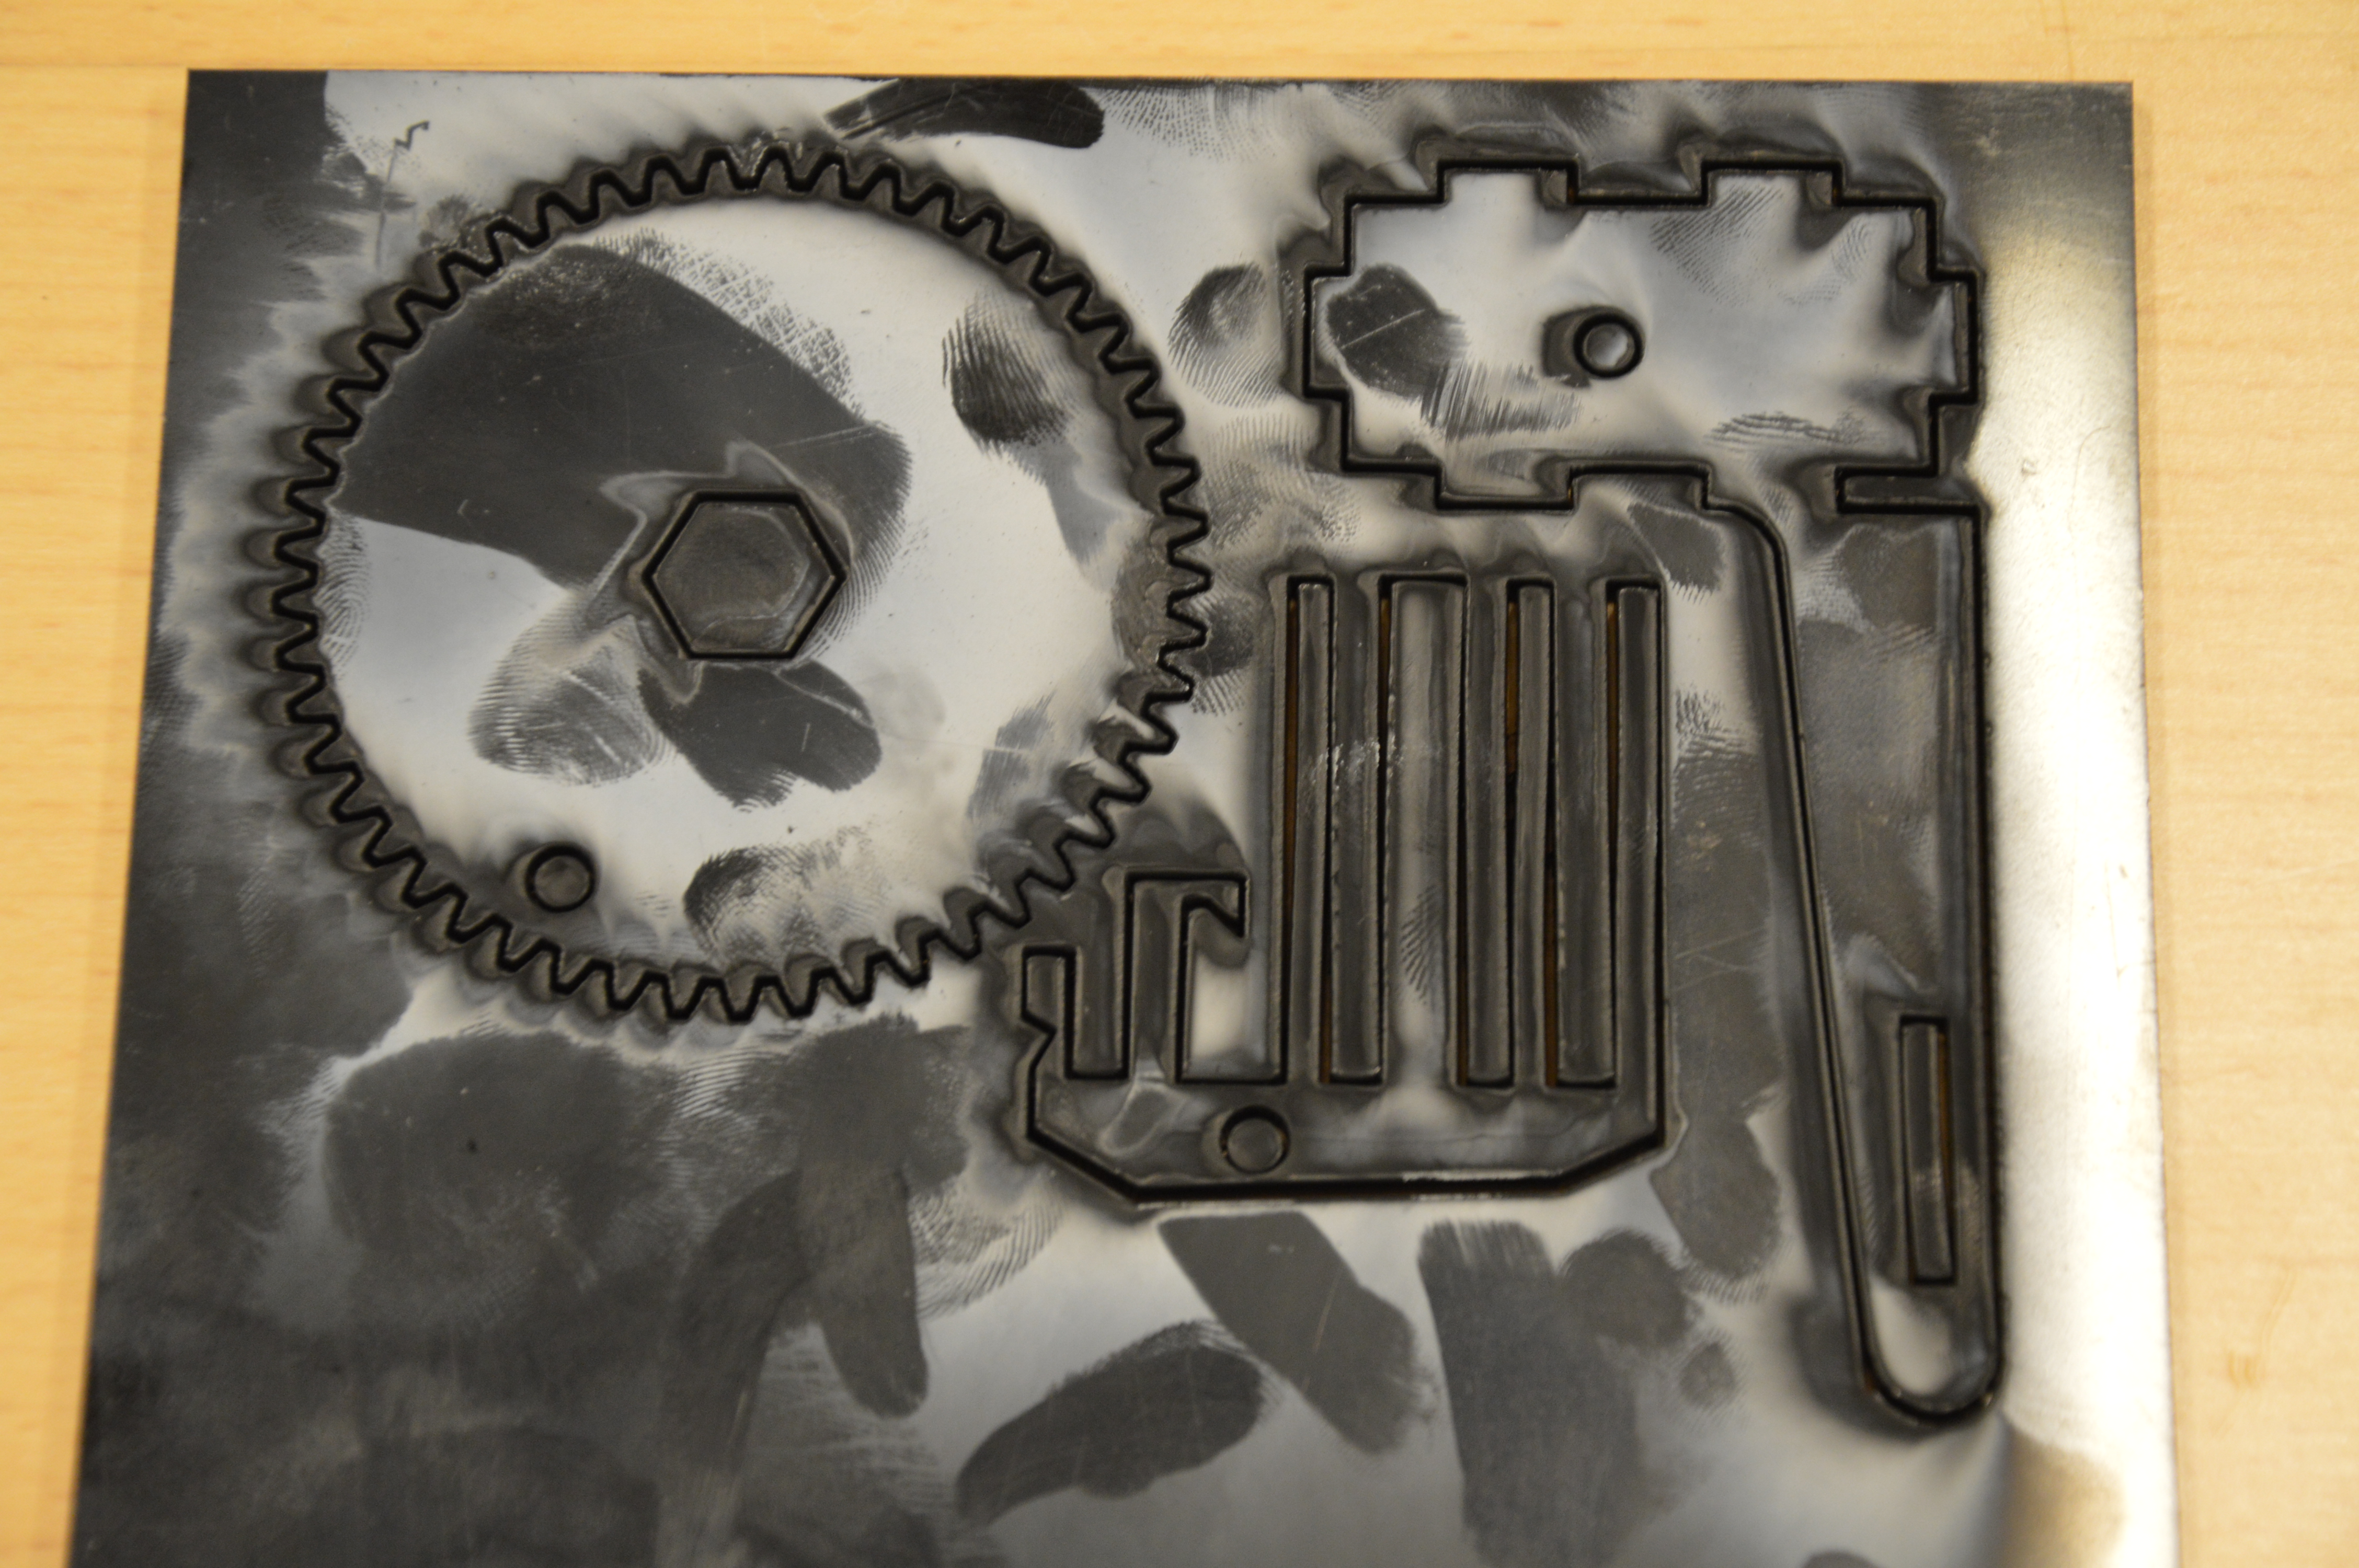
\includegraphics[scale=0.1]{images/DSC_0048.JPG}
		\caption{\small {\it {This is a description}}} \label{fig:explode}
	\end{center}
\end{figure}

RIALEN PP
\begin{figure}[h]
	\begin{center}
		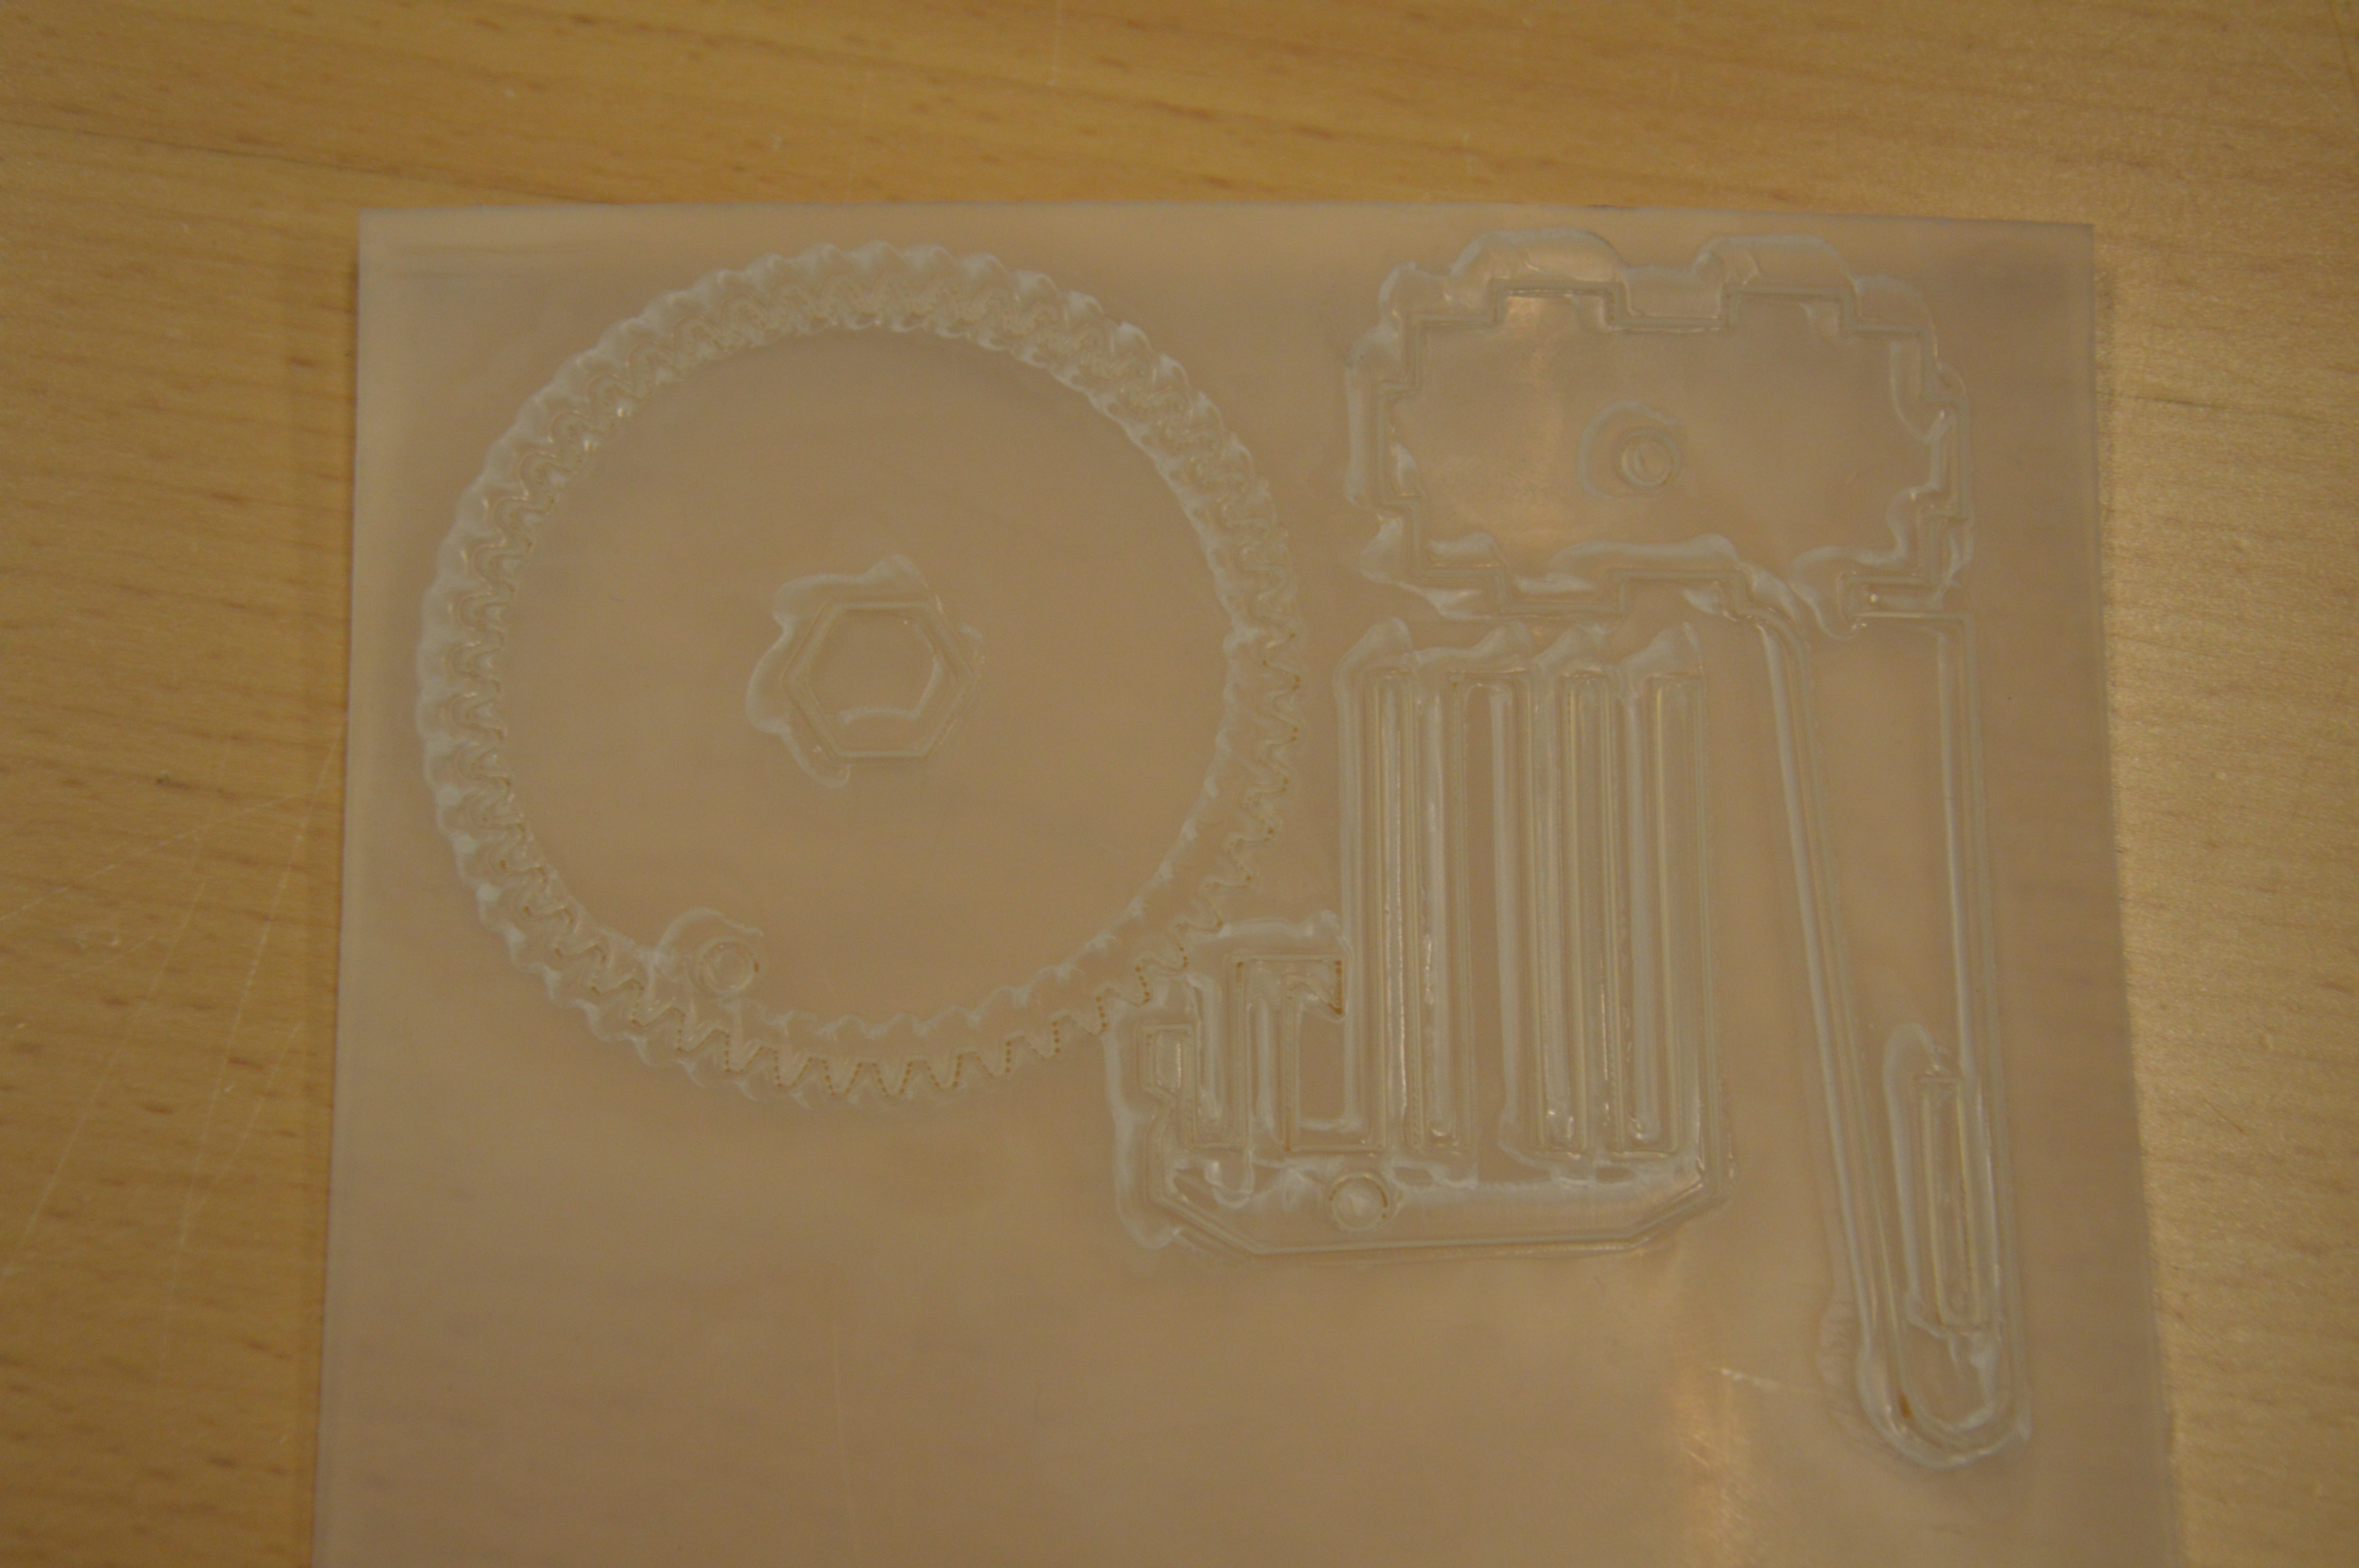
\includegraphics[scale=0.1]{images/DSC_0053.JPG}
		\caption{\small {\it {This is a description}}} \label{fig:explode}
	\end{center}
\end{figure}
PETG
\begin{figure}[h]
	\begin{center}
		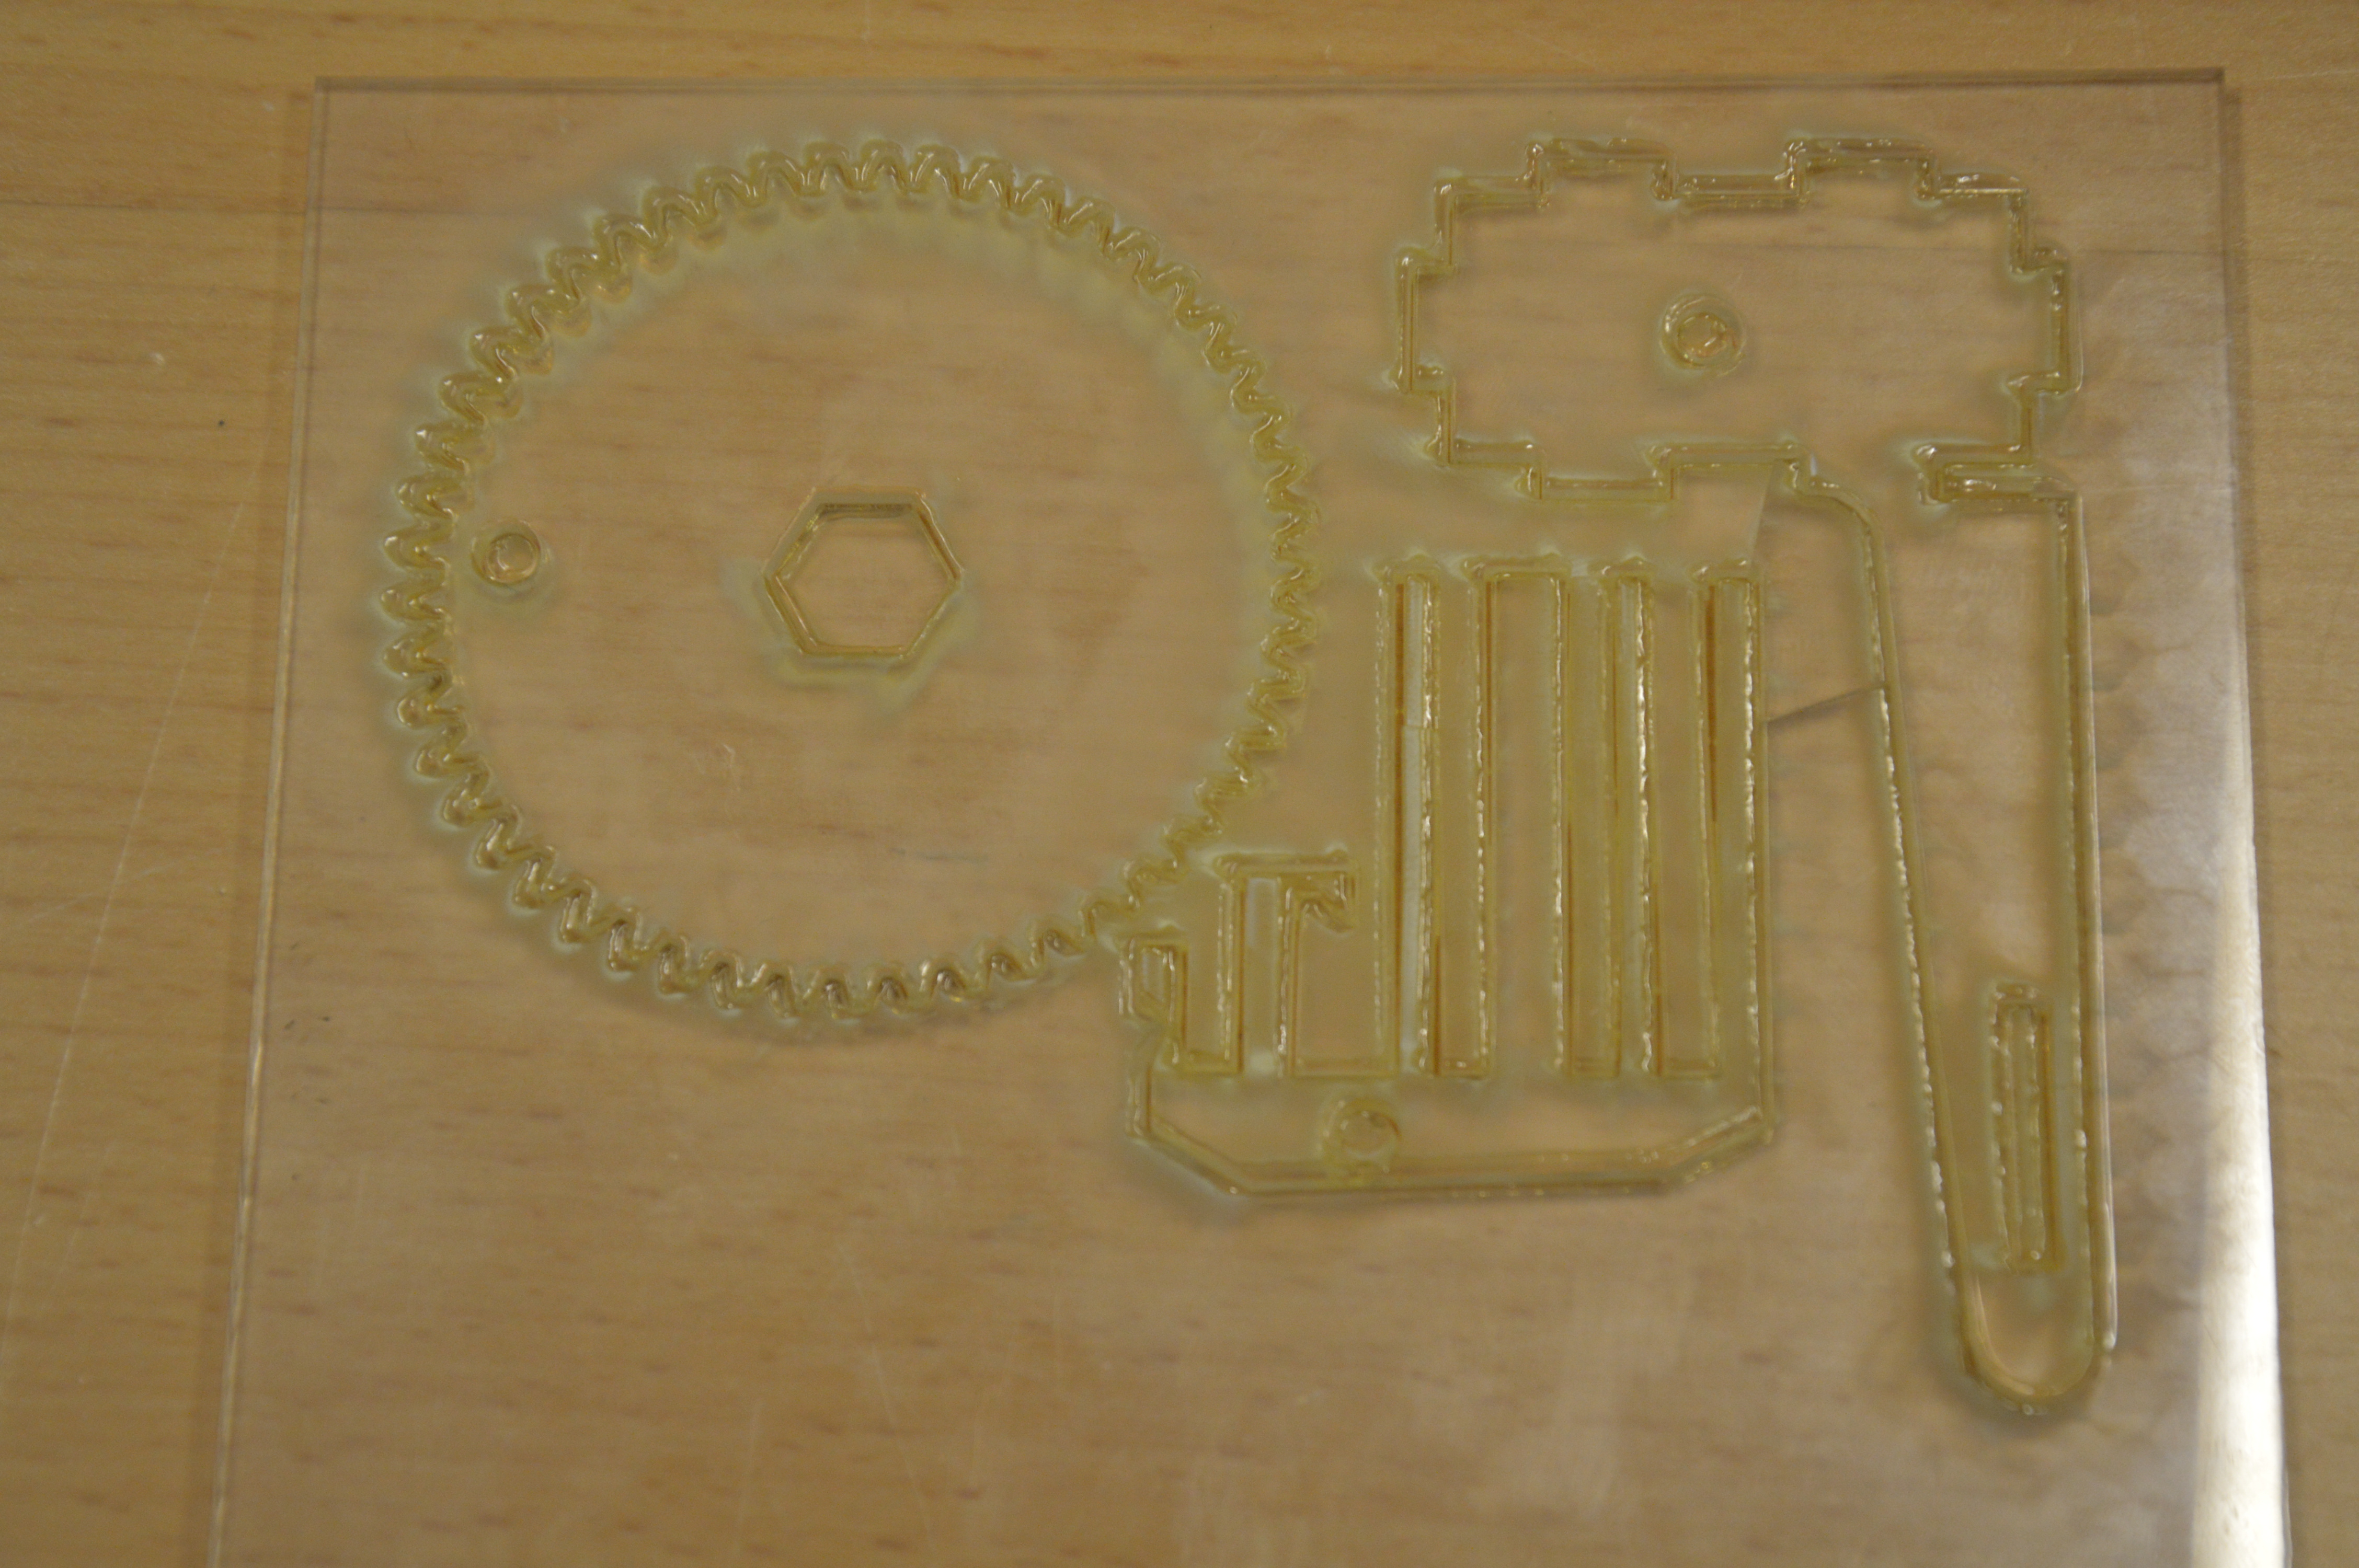
\includegraphics[scale=0.1]{images/DSC_0023.JPG}
		\caption{\small {\it {This is a description}}} \label{fig:explode}
	\end{center}
\end{figure}
PP-H
\begin{figure}[h]
	\begin{center}
		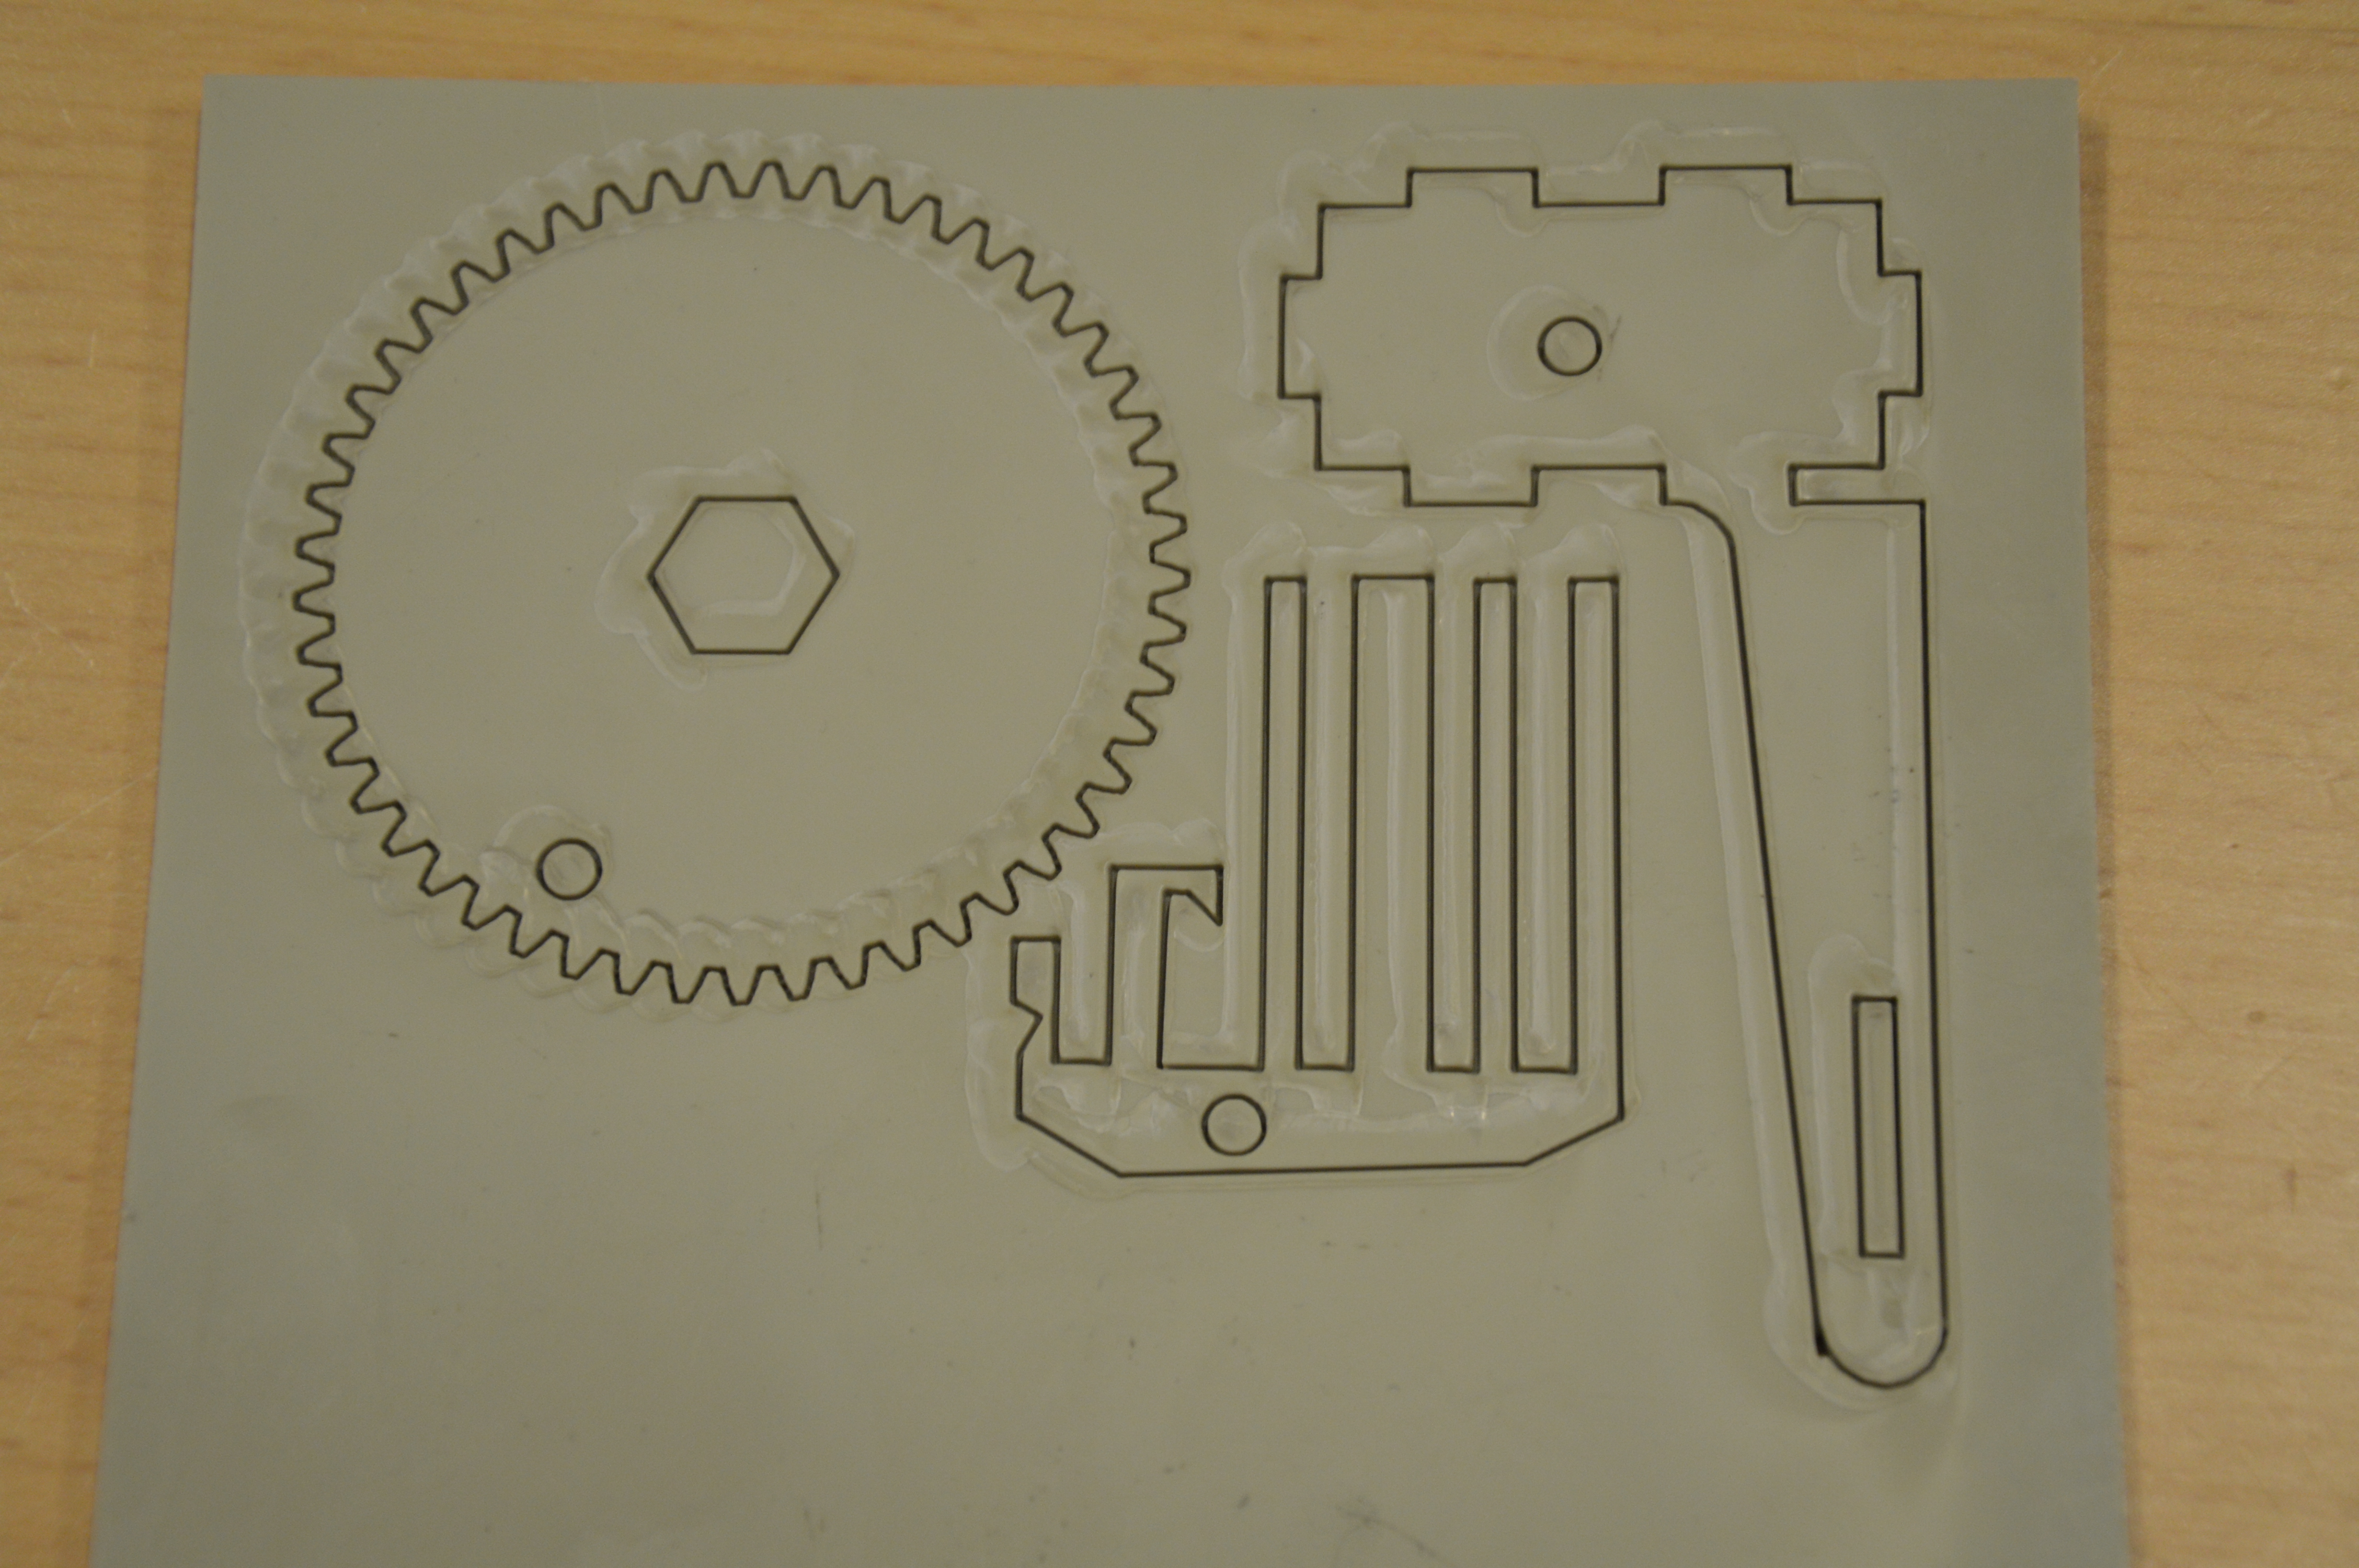
\includegraphics[scale=0.1]{images/DSC_0029.JPG}
		\caption{\small {\it {This is a description}}} \label{fig:explode}
	\end{center}
\end{figure}
POM-C
\begin{figure}[h]
	\begin{center}
		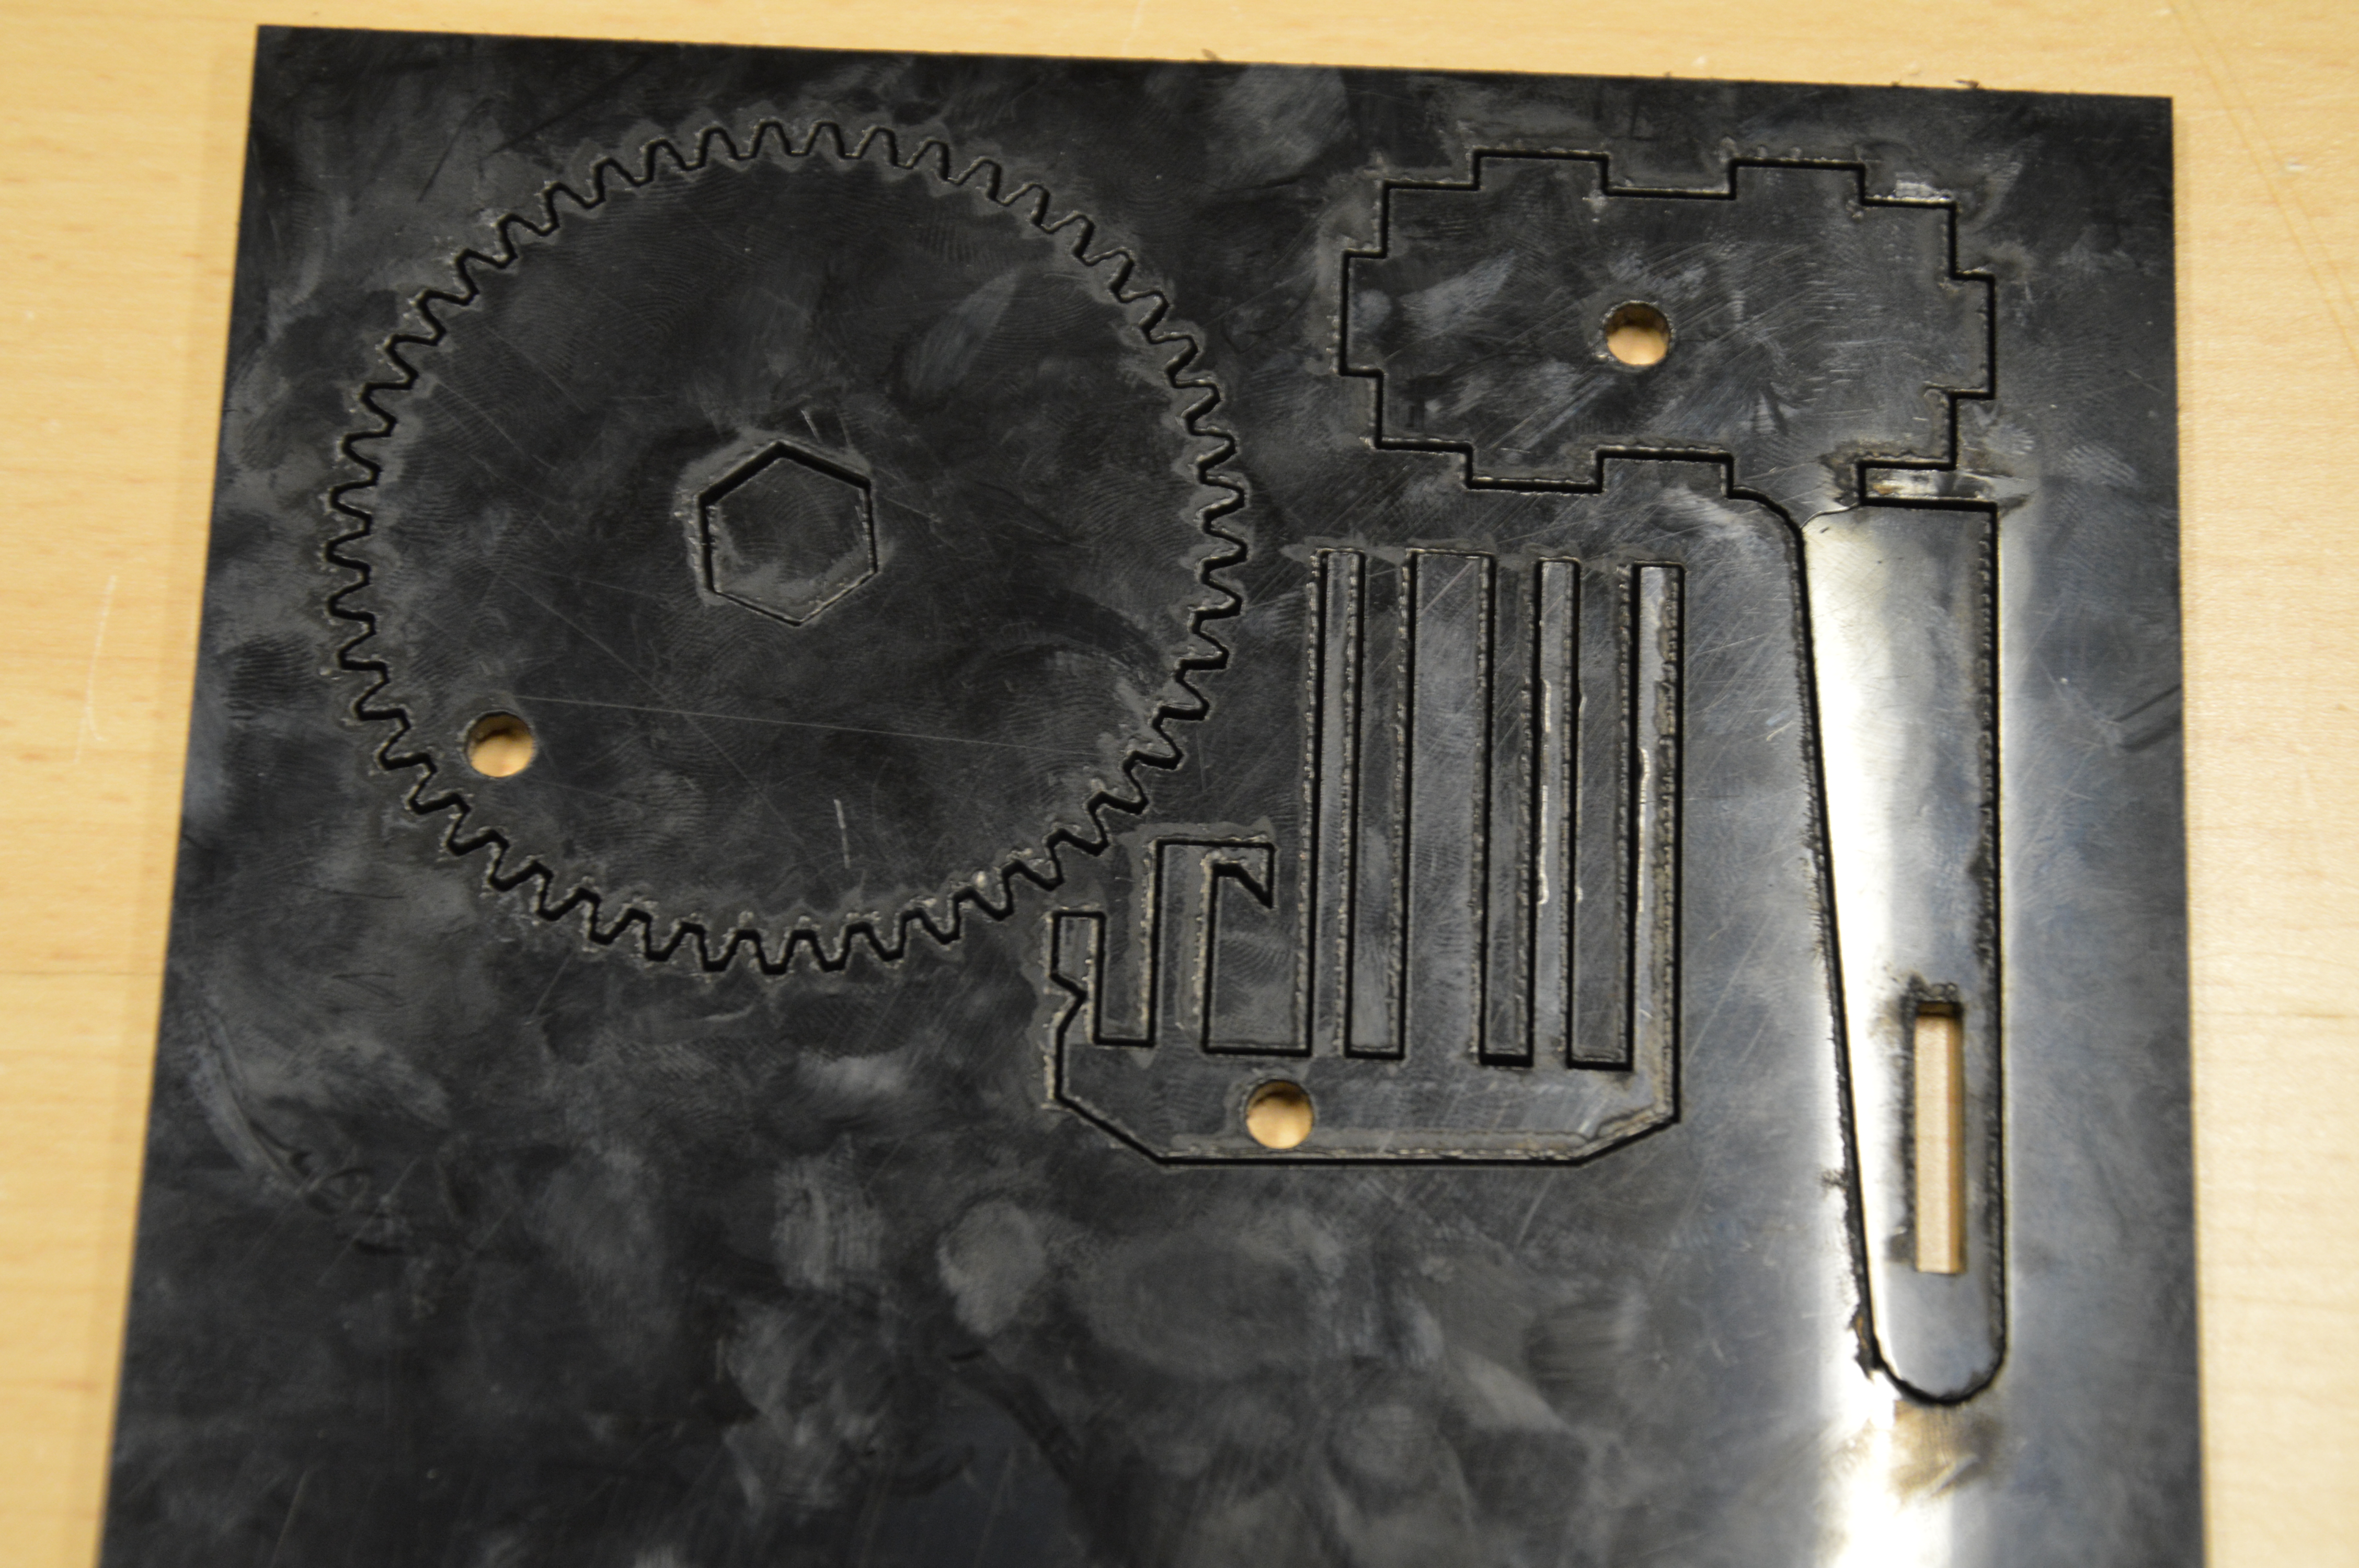
\includegraphics[scale=0.1]{images/DSC_0039.JPG}
		\caption{\small {\it {This is a description}}} \label{fig:explode}
	\end{center}
\end{figure}

ACRYL
PEEK
PPSU

\subsection{Iterations}
we have used prototyping in order to get a viable device, through the different designs we have been able to see different problems, which have ment that we had to iterate to a new version, we have been limited by time, so we have had to make some compromises

\subsubsection{fisrt}
The first iteration that we build did have some problems.
The first is that it is expensive to build, since we are using a lot of acrylic, the secound point is that it still is heavy, and unwieldy.
But i did give some ideas for the next iteration.

\subsubsection{secound}


\subsubsection{thried}


\subsubsection{fourth}


\subsubsection{fith}

\subsubsection{sixth}

